\documentclass{article}

% if you need to pass options to natbib, use, e.g.:
% \PassOptionsToPackage{numbers, compress}{natbib}
% before loading nips_2016
%
% to avoid loading the natbib package, add option nonatbib:
% \usepackage[nonatbib]{nips_2016}

%\usepackage{nips_2016}
\usepackage[final]{nips_2016}

% to compile a camera-ready version, add the [final] option, e.g.:
%\usepackage[final]{nips_2016}

\usepackage[utf8]{inputenc} % allow utf-8 input
\usepackage[T1]{fontenc}    % use 8-bit T1 fonts
\usepackage{hyperref}       % hyperlinks
\usepackage{url}            % simple URL typesetting
\usepackage{booktabs}       % professional-quality tables
\usepackage{amsfonts}       % blackboard math symbols
\usepackage{nicefrac}       % compact symbols for 1/2, etc.
\usepackage{microtype}      % microtypography
\usepackage{graphicx}	%inserting images

\title{Self-driving vehicle in Duckietown environment\\
	\large Duckpropagation }

% The \author macro works with any number of authors. There are two
% commands used to separate the names and addresses of multiple
% authors: \And and \AND.
%
% Using \And between authors leaves it to LaTeX to determine where to
% break the lines. Using \AND forces a line break at that point. So,
% if LaTeX puts 3 of 4 authors names on the first line, and the last
% on the second line, try using \AND instead of \And before the third
% author name.

\author{
  Attila Pethő
 % \texttt{hippo@cs.cranberry-lemon.edu} \\
  %% examples of more authors
   \And  
   Farkas Olivér István \\
  %% Affiliation \\
  %% Address \\
  %% \texttt{email} \\
   \And
    Faragó Gyula\\
  %% Affiliation \\
  %% Address \\
  %% \texttt{email} \\
  %% \And
  %% Coauthor \\
  %% Affiliation \\
  %% Address \\
  %% \texttt{email} \\
  %% \And
  %% Coauthor \\
  %% Affiliation \\
  %% Address \\
  %% \texttt{email} \\
}

\begin{document}
% \nipsfinalcopy is no longer used

\maketitle

\begin{abstract}
  In this project we are training Deep Reinforcement Learning agents to drive small robots called Duckiebots in the Duckietown environment. There are four challenges in the environment:

\textbullet  \textbf{LF} - simple lane following\\
\textbullet \textbf{LFV} - lane following with vehicles\\
\textbullet \textbf{LFI} - lane following with intersections\\
\textbullet \textbf{LFVI} - lane following with vehicles and intersections\\
In order to conquer these challenges, autonomous driving agents are first trained in a simulator (gym-duckietown) and then the trained agents performance are also tested in the real environment on real Duckiebots.
\end{abstract}

\section{\large{Introduction}}

Self driving vehicles are clearly the future of transportation. If you look at waymo's  (https://waymo.com/safety/) safety report you can see two things. First its obvious that it's more safe than a human driven vehicle. The other thing which makes development hard is the amount of data needed for the training of the AI.

\bigbreak

Duckietown has started in a class at MIT in 2016. Duckietown has grown so much since then, it's now a worldwide initiative to learn AI and robotics.

\section{\large{Installation}}

\textbf{Requirements: git installed on your computer}

You need to clone the following repository:\\
\begin{center}
  \url{https://github.com/attila-petho/DuckPropagation}
\end{center}

If you are done with that, change directory into DuckPropagation with the following command:
\begin{center}
	cd DuckPropagation/
\end{center}
After that you need to run the script that sets up the environment:
\begin{center}
	bash env\_setup.sh
\end{center}

\section{\large{Methods}}

\subsection{\normalsize{RL}}

\begin{figure}[h!]
	\centering
	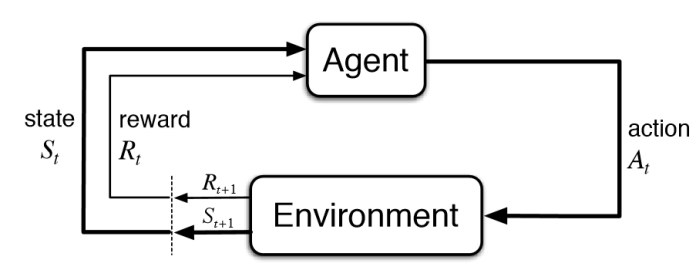
\includegraphics[width=0.8\linewidth]{rl.jpg}
	\caption{Illustration of Reinforcement Learning}
\end{figure}

\subsection{\normalsize{A2C, PPO algorithms}}

\subsection{\normalsize{Environment}}

The environment gives us an 640x480 RGB image which looks like the following:
\begin{figure}[h!]
	\centering
	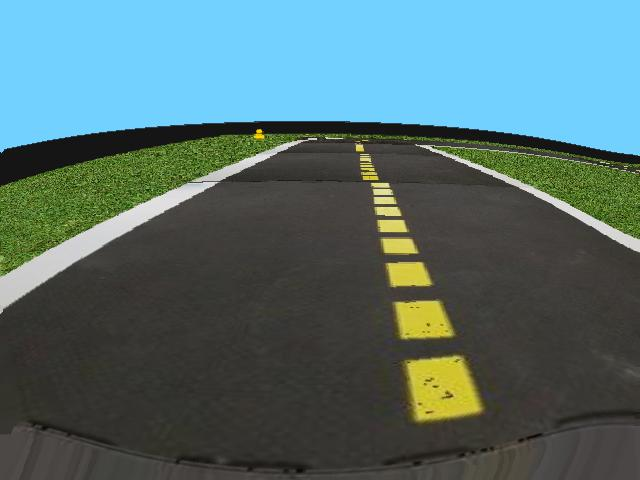
\includegraphics[width=0.5\linewidth]{rawobs.jpg}
	\caption{Observation of the environment without preprocessing}
\end{figure}
We have to preprocess this image, because feeding the original images to the CNN would be a waste of resources because it makes training process much slower, and the network can learn from smaller images just as well. We did the following preprocessing steps:
\begin{enumerate}
	\item Resizing
	\item Cropping
	\item Color segmentation or Grayscaling
	\item Normalization
	\item Frame stacking
\end{enumerate}
\subsubsection{\normalsize{Observations}}
In this section we will present our environment wrappers which return the observations.
\textbullet  \textbf{ResizeFrame}\\
With this wrapper we are downscaling the images from their original size (480x640x3) to (84x84x3). The smaller dimension makes the training of the neural network faster, and it still carries enough information for efficient training.\\
\textbullet  \textbf{CropFrame}\\
In this wrapper we are cropping the useless information from the image, in our case it's the part above the horizon.\\
\begin{figure}[h!]
	\centering
	\begin{minipage}{.5\textwidth}
	\centering
	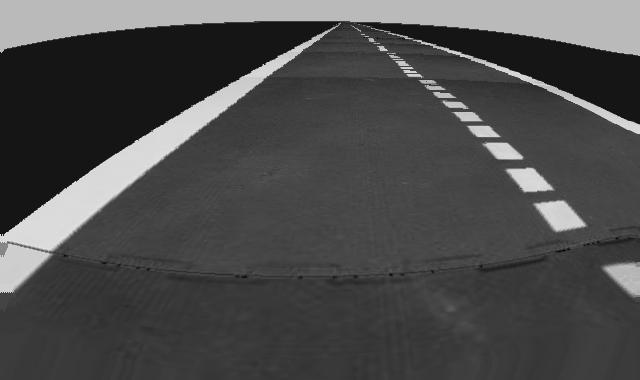
\includegraphics[width=0.8\linewidth]{grayscale.jpg}
	\caption{Observation from the environment with grayscaling}
	\end{minipage}%
\begin{minipage}{.5\textwidth}
	\centering
	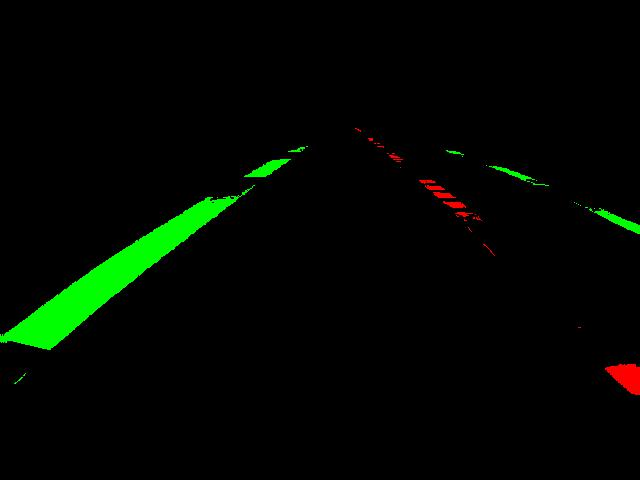
\includegraphics[width=0.8\linewidth]{colorseg.jpg}
	\caption{Observation from the environment with color segmentation}
\end{minipage}
\end{figure}
\textbullet  \textbf{GrayScaleFrame}\\
Training time can be reduced by using grayscale images instead of RGB, while keeping the important information of the images. This wrapper should not be used in conjunction with the ColorSegmentFrame wrapper.\\

\textbullet  \textbf{ColorSegmentFrame}\\
Here we are segmenting the different parts of the image so we can feed the neural network more useful information. The segmentation is done using intervals, we assigned the red channel for the white line, and the green channel for the yellow line. For lane following only these two information are useful for the neural network, so we assign black for everything else.\\
\textbullet  \textbf{NormalizeFrame}\\
To make the training of the CNN easier and faster this wrapper normalizes the pixel values in the interval of [0,1]. Altough we implemented this wrapper, it is not used, because stable baselines does the input normalization automatically.\\
\textbullet  \textbf{StackFrame}
For better quality in training and more information we are concatenating the last n frames to form a time series, so the agent can percieve dynamic changes in its environment.\\

\subsubsection{\normalsize{Actions}}

\subsubsection{\normalsize{Rewards}}

\subsection{\normalsize{Evaluation}}

\subsection{\normalsize{Hyperparameter Optimization}}

\section{\large{Results}}

\section{\large{Conclusion}}

\section*{References}

\small

[1] András Kalapos, Csaba Gór, Róbert Moni and István Harmati. "Sim-to-real reinforcement learning applied to end-to-end vehicle control" arXiv:2012.07461
(2020) (\url{https://github.com/kaland313/Duckietown-RL})


\end{document}